\clearpage
\section{Experiment: Position-Angle}

Cleveland and McGill measure human perception of quantities encoded as positions and as angles through their position-angle experiment~\cite{cleveland_mcgill}. The actual experiment compares pie charts versus bar charts since these map down to elementary position and angle judgement. We create rasterized images mimicking Cleveland and McGill's proposed encoding and investigate computational perception of our four networks.

We follow the data generation according to Cleveland and McGill and generate datasets of 5 numbers which add to 100. The numbers fulfill their proposed requirements of being greater than 3 smaller than 39, with differences between values being greater than $0.1$. Similar to Cleveland and McGill, we create pie chart and bar chart representations (Fig.~\ref{fig:figure3_mlae}, left). We create these visualizations as $100\times100$ pixel raster images. We then mark the largest quantitiy of the five in each visualization with a single pixel dot. The regression task, again similar to the experiment bei Cleveland and McGill, is to estimate what value each quantity is in relation to the marked largest. Since the position of the largest element changes, we generate the targets in such fashion that the largest element is marked with 1 and the other quantities follow counter-clockwise for the pie chart and to the right for the bar chart. To be successful, the networks essentially first have to find the marked quantity, have the `rolling' encoding figured out, and then estimate the quantities properly. We generate the pie chart and bar chart visualizations with $878,520$ possible permutations each which renders this regression task as a decent problem.

%\begin{figure}[t]
%	  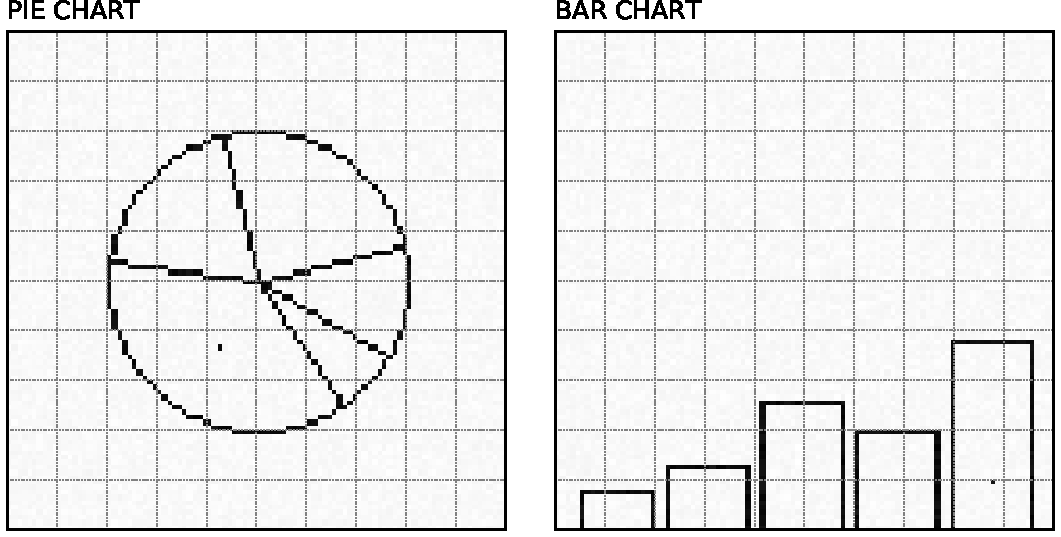
\includegraphics[width=\linewidth]{figure3_overview}
%  \caption{\textbf{Position-Angle Experiment.} We create rasterized visualizations of pie charts and bar charts to follow Cleveland and McGill's position-angle experiment. The experimental task involves the judgement of different encoded values in comparison to the largest encoded values. The pie chart (left) and the bar chart (right) visualize the same data point. In their paper, Cleveland and McGill report less errors using bar charts.}
%	\label{fig:position_angle_experiment}
%\end{figure}
%\begin{table}[h]
%\centering
%\caption{\textbf{Position-Angle Experiment.} We create rasterized visualizations of pie charts and bar charts to follow Cleveland and McGill's position-angle experiment. The experimental task involves the judgement of different encoded values in comparison to the largest encoded values. The pie chart and the bar chart visualize the same data point. In their paper, Cleveland and McGill report less errors using bar charts.}
%\resizebox{\linewidth}{!}{
%\begin{tabular}{lllr}
%	\toprule
%	\multicolumn{2}{l}{~} & ~ & Permutations\\
%
%	\midrule
%	\raisebox{-.85\height}{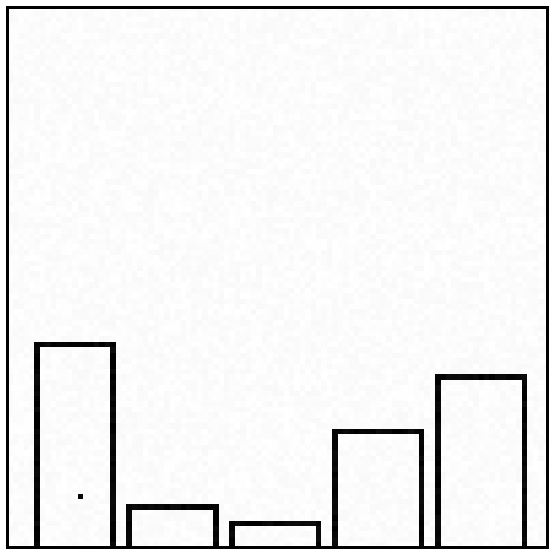
\includegraphics[width=.5in]{figure3_Bar_Chart.pdf}} & \makecell[tl]{Type 1: \emph{Bar Chart}\\~~~Perceptual Task: \emph{Position}\\~ \\~ \\} &~& \makecell[tr]{~\\ $878,520$}\\
%
%
%	\midrule
%	\raisebox{-.85\height}{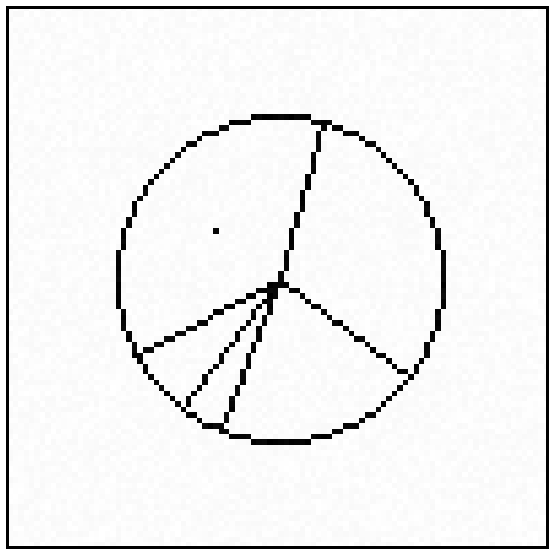
\includegraphics[width=.5in]{figure3_Pie_Chart.pdf}} & \makecell[tl]{Type 2: \emph{Pie Chart}\\~~~Perceptual Task: \emph{Angle}\\~ \\~ \\} &~& \makecell[tr]{~\\ $878,520$}\\
%
%
%	\bottomrule
%\end{tabular}
%}
%\label{tab:pos_angle_parameters}
%\end{table}

\subsection{Hypotheses}

We proposed two hypotheses entering the elementary perceptual task experiment:

\begin{itemize}
	\item \textbf{H2.1} \textbf{Computed perceptual performance is better using bar charts than pie charts.} Cleveland and McGill report that position judgements are almost twice as accurate as angle judgements. This renders bar charts superior to pie charts and should also be the case for convolutional neural networks.
	\item \textbf{H2.2} \textbf{Convolutional neural networks can learn position faster than angles.} We assume that regressing bar charts is easier than understanding pie charts. Following our ranking of elementary perceptual tasks (Table~\ref{tab:ranking}), we suspect that our networks learn encodings of positions faster than angles resulting in more efficient training and faster convergence.
\end{itemize}

\subsection{Results}

\begin{figure}[t]
	\centering
	  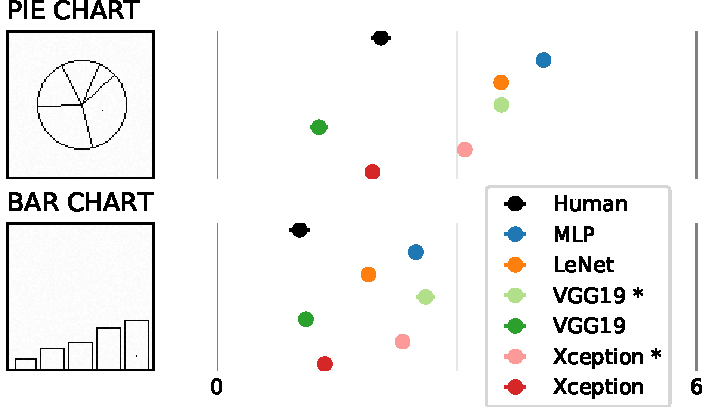
\includegraphics[width=\linewidth]{figure3_mlae_better_all.pdf}
  \caption{\textbf{Computational results of the position-angle experiment.} \textit{Left:} Our encodings of one data point as a pie chart and a bar chart. \textit{Right:} MLAE and 95\% confidence intervals for different networks. VGG19 * and Xception * are using ImageNet weights while all other networks were trained on the stimuli. We mimmick the original experiment of Cleveland and McGill and compare against their human results~\cite{cleveland_mcgill}.}
	\label{fig:figure3_mlae}
\end{figure}

\noindent{\textbf{Perceptual Performance.}} Our networks are able to perform the regression task for bar charts and for pie charts (Fig.~\ref{fig:figure3_mlae}). We evaluate over 56 runs for each condition \textit{visual encoding} (12 runs per network, but only 4 for VGG19 and Xception due to higher training times), which yields an average $MLAE=2.176$ for bar chart ($SD=0.456$), and $3.296$ ($SD=0.77$) for pie chart. This difference is statistically significant ($F_{1,110}=86.061, p<0.01$) and leads us to \textbf{accept H2.1}. Post hoc comparisons show that this holds for most networks: 
MLP for pie charts $4.09$ ($SD=0.027$) and for bar charts $2.494$ ($0.068$) is significant ($t_{22}=72.300,p<0.01$), 
LeNet for pie charts $ 3.556 $ ($SD= 0.022 $) and for bar charts $ 1.902 $ ($SD= 0.08 $) is significant $t_{22}=66.111, p<0.01$, 
VGG19 *  for pie charts $ 3.561 $ ($SD= 0.047 $) and for bar charts $ 2.601 $ ($SD= 0.113 $) is significant $t_{22}=25.919,p<0.01$, 
Xception * for pie charts  $ 3.094 $ ($SD= 0.046 $) and for bar charts $ 2.315 $ ($SD= 0.032 $) is significant $t_{22}=46.329,p<0.01$, 
and Xception for pie charts $ 1.939 $ ($SD= 0.1 $) and for bar charts $ 1.375 $ ($SD= 0.062 $) is significant $t_{22}=8.276,p<0.01$.
The difference for VGG19 (pie charts $ 1.297 $ ($SD= 0.129 $), bar charts $ 1.153 $ ($SD= 0.09 $)) was not significant with $p<0.05$. This is not surprising since VGG19 is a very powerful network which can adapt to seemingly any visual encoding as seen in our ranking for elementary perceptual tasks (Table~\ref{tab:ranking}).
\\~\\
\noindent{\textbf{Training Efficiency.} We measure the MSE loss for all networks on previously unseen validation data during training. We count a network as converged when this validation loss does not decrease after 10 sequential epochs meaning that each network and even each run stops after a varying number of training epochs. To measure the training efficiency, we look at the MSE validation loss during the first twenty epochs of 56 runs for each condition. Visually inspected, the pie chart loss decreases slower (Fig.~\ref{fig:figure3_val_loss}). The average loss in this period is for pie charts $0.052$ ($SD=0.015$) and for bar charts $0.037$ ($SD=0.018$). This difference is statistically significant ($F_{1,2238}=20.656, p<0.01$). We therefor conclude that networks train more efficiently and faster when learning bar charts and \textbf{accept H2.2}. 
\\~\\
It seems that the visual encoding of bar charts is superior to pie charts in terms of performance and efficiency. This is interesting since Cleveland and McGill observe the same effect during their human experiment and conclude that the perceptual task of estimating position is easier for humans than the estimation of angles. Our ranking of elementary perceptual tasks yields a low score for angles and the related encoding of directions while position ranks in the mid to top.

\begin{figure}[t]
	  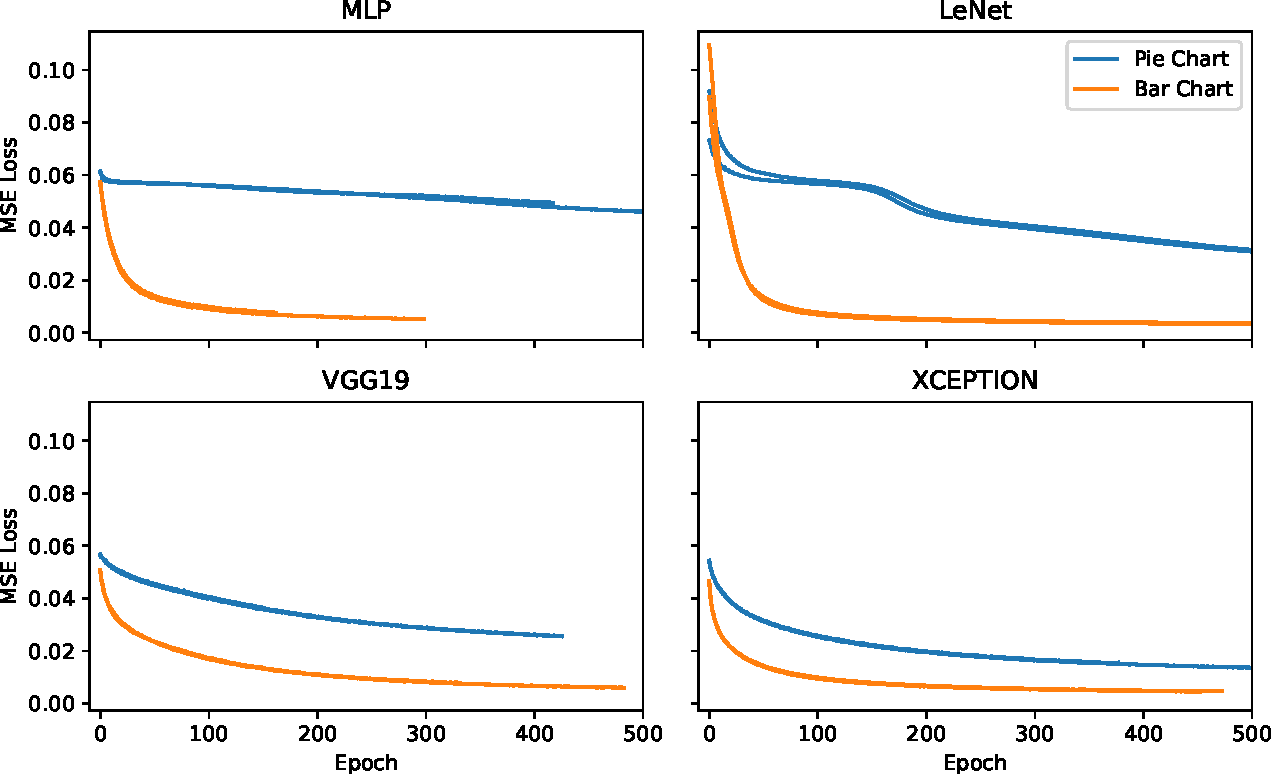
\includegraphics[width=\linewidth]{figure3_val_loss.pdf}
  \caption{\textbf{Training efficiency of the position-angle experiment.} Mean Squared Error (MSE) loss during training of our networks computed on previously unseen validation data after each epoch. The regressors estimate quantities in pie charts and bar charts. We train all networks 12 times (4 times for VGG19 and Xception due to longer training times). VGG19 * and Xception * use ImageNet weights. All networks converge faster when learning bar charts.}
	\label{fig:figure3_val_loss}
\end{figure}

